\documentclass[aip,adv,reprint,floatfix]{revtex4-2}

\usepackage{amsmath, amssymb, amsfonts}
\usepackage{physics}
\usepackage{tikz}
\usepackage{graphicx}
\usepackage{hyperref}
\usetikzlibrary{arrows.meta,calc,positioning,patterns}
\definecolor{accent}{RGB}{11,93,104}

\begin{document}

\title{Displacement-Engineered Warp Fields: Tic-Tac Geometry, Stability Surfaces, and Identity-Space Confinement}

\author{Jason Dutton}
\affiliation{Independent Theoretical Researcher, Castlewood, Virginia, USA}

\date{\today}

\begin{abstract}
Recent publicly reported aerospace observations describing smooth, capsule-like craft exhibiting extreme kinematic profiles have renewed interest in geometric models capable of representing unconventional motion signatures. Although such reports do not constitute physical evidence of novel propulsion systems, they motivate the development of conceptual engineering frameworks grounded in geometric field theory; the present paper is therefore a model proposal, not a claim that the reported observations establish a vehicle or mechanism. Public UAP reporting and its evidentiary limits are summarized by NASA~\cite{NASA2023UAP}. In this work, we present a displacement-based warp-field model constructed within the identity-space formalism of the Single Entity Field Interpretation (SEFI), Dynamic Entity Field Integration (DEFI), and the Geometric Worldline Field Model (GWFM)~\cite{DuttonSEFI2026,DuttonGWFM2026,DuttonUnified2026}. The model treats the ``tic-tac'' craft as a well-defined engineering object with capsule geometry, boundary-layer confinement, displacement amplitudes, gradient constraints, and stability surfaces. We derive the governing equations for displacement fields, establish curvature and torsion limits preventing worldline intersection, and construct a flight-envelope inequality bounding effective motion. The resulting framework is a falsifiable mathematical specification for evaluation, critique, and extension by researchers in geometric field theory, aerospace engineering, and applied physics.
\end{abstract}

\maketitle
\section{Introduction}

Recent publicly reported aerospace observations have described smooth, capsule-like craft exhibiting extreme kinematic profiles, including rapid displacement, abrupt changes in trajectory, and high-acceleration motion without conventional aerodynamic signatures. Although such reports do not constitute physical evidence of novel propulsion systems, they motivate the development of conceptual engineering frameworks capable of representing unconventional motion signatures within a mathematically coherent structure. The present work adopts this motivation in a strictly formal context, constructing a displacement-based warp-field model grounded in geometric field theory.

The Single Entity Field Interpretation (SEFI), Dynamic Entity Field Integration (DEFI), and the Geometric Worldline Field Model (GWFM) provide the underlying mathematical foundation for the present analysis~\cite{DuttonSEFI2026,DuttonGWFM2026,DuttonUnified2026}. These frameworks treat worldlines as geometric objects embedded within identity-space, subject to displacement operators, stability surfaces, and curvature constraints. Within this formalism, motion is represented not as acceleration through spacetime but as a displacement of worldlines under a smooth operator $\mathcal{D}$ acting on the identity-space manifold. This approach is deliberately kinematic: it does not supply a stress-energy source, propulsion mechanism, or experimental validation, and it should not be confused with metric-engineering proposals such as the Alcubierre spacetime~\cite{Alcubierre1994} or traversable-wormhole analyses~\cite{MorrisThorne1988}.

The tic-tac craft is modeled as a well-defined engineering object with capsule geometry, smooth curvature, and a confined boundary layer. The geometry is selected to match publicly reported dimensions: a length of approximately $14\,\mathrm{m}$, a maximum radius of $2\,\mathrm{m}$, and a boundary-layer thickness of $1\,\mathrm{m}$. These values are incorporated into the displacement-field construction and stability-surface analysis; the geometry and its boundary layer are summarized in Fig.~\ref{fig:capsule_geometry}. The resulting model provides a structured engineering specification for a displacement-based vehicle, suitable for evaluation by researchers in geometric field theory, aerospace engineering, and applied physics.

The objectives of this work are threefold. First, to define a displacement field $\Delta(\mathbf{x})$ capable of producing effective motion without violating local relativistic constraints. Second, to establish gradient, curvature, and torsion limits preventing worldline intersection and ensuring identity-space coherence. Third, to construct a flight-envelope inequality bounding effective displacement per unit ambient time. The analysis is supplemented by an engineering appendix detailing geometric parameters, boundary-layer structure, displacement amplitudes, and stability-surface tolerances.

The remainder of this paper is organized as follows. Section III introduces the geometric framework and displacement operator. Section IV defines the tic-tac craft geometry and boundary-layer confinement. Section V derives the displacement field and its governing equations. Section VI establishes stability surfaces and gradient constraints. Section VII constructs the flight-envelope inequality. Section VIII presents engineering requirements and operational considerations. Section IX provides concluding remarks. An appendix contains detailed geometric specifications and parameter tables.
\section{Geometric Framework}

The displacement-based warp-field model developed in this work is constructed within the identity-space formalism established in the Single Entity Field Interpretation (SEFI), Dynamic Entity Field Integration (DEFI), and the Geometric Worldline Field Model (GWFM). In this section, we summarize the geometric structure required for the displacement operator, the representation of worldlines, and the constraints necessary to preserve identity-space coherence.

\subsection{Identity-Space Manifold}

Identity-space is modeled as a smooth, connected, four-dimensional differentiable manifold $\mathcal{I}$ equipped with a metric-compatible affine connection. Each physical entity is represented by a worldline $\gamma : \mathbb{R} \rightarrow \mathcal{I}$, where $\gamma(\tau)$ denotes the identity-space position of the entity at ambient parameter $\tau$. The manifold admits a decomposition into spatial coordinates $\mathbf{x} \in \mathbb{R}^3$ and an identity coordinate $\sigma \in \mathbb{R}$, yielding local charts $(\mathbf{x},\sigma)$ suitable for displacement-field construction.

The connection $\nabla$ defines curvature $\kappa$ and torsion $\tau$ along worldlines, with
\begin{equation}
\kappa = \left\| \nabla_{\dot{\gamma}} \dot{\gamma} \right\|,
\qquad
\tau = \left\langle \nabla_{\dot{\gamma}} B, N \right\rangle,
\end{equation}
where $B$ and $N$ denote binormal and normal vectors of the Frenet frame. These quantities are used to establish curvature and torsion limits preventing worldline intersection under displacement.

\subsection{Worldline Representation}

A worldline $\gamma(\tau)$ is represented as a curve in identity-space with tangent vector $\dot{\gamma}(\tau)$ and second derivative $\ddot{\gamma}(\tau)$ defined with respect to the ambient parameter. Classical motion corresponds to smooth evolution of $\gamma(\tau)$ under the connection $\nabla$. In contrast, displacement-based motion is represented by the action of a displacement operator $\mathcal{D}$ acting on $\gamma$:
\begin{equation}
\gamma'(\tau) = \mathcal{D}\big(\gamma(\tau)\big).
\end{equation}
The operator $\mathcal{D}$ is constructed to be smooth, invertible, and confined within a boundary layer surrounding the craft geometry. This ensures that worldlines remain continuous and non-intersecting under displacement.

\subsection{Displacement Operator}

The displacement operator is defined as
\begin{equation}
\mathcal{D}(\mathbf{x}) = \mathbf{x} + \Delta(\mathbf{x}),
\end{equation}
where $\Delta(\mathbf{x})$ is a smooth displacement field satisfying gradient, curvature, and torsion constraints. The displacement amplitude $\Delta_0$ is defined as
\begin{equation}
\Delta_0 = \max_{\mathbf{x}} \left\| \Delta(\mathbf{x}) \right\|,
\end{equation}
and the displacement gradient is given by
\begin{equation}
\nabla \Delta = \left( \frac{\partial \Delta_i}{\partial x_j} \right).
\end{equation}
To prevent worldline intersection, the gradient must satisfy
\begin{equation}
\left\| \nabla \Delta \right\| \leq G_{\max},
\end{equation}
where $G_{\max}$ is a stability-surface parameter determined in Section VI.

\subsection{Non-Intersection Constraints}

Identity-space coherence requires that worldlines remain distinct under displacement. This imposes the constraint
\begin{equation}
\gamma_1'(\tau) \neq \gamma_2'(\tau)
\qquad
\forall \tau, \quad \forall \gamma_1 \neq \gamma_2,
\end{equation}
which is satisfied if the displacement field obeys
\begin{equation}
\left\| \Delta(\mathbf{x}_1) - \Delta(\mathbf{x}_2) \right\|
\geq
\epsilon \left\| \mathbf{x}_1 - \mathbf{x}_2 \right\|,
\end{equation}
for some $\epsilon > 0$ determined by the stability surface. This condition ensures that displacement does not collapse distinct worldlines into a single identity-space location.

\subsection{Curvature and Torsion Limits}

To prevent geometric singularities, the curvature and torsion of displaced worldlines must satisfy
\begin{equation}
\kappa' \leq \kappa_{\max},
\qquad
\tau' \leq \tau_{\max},
\end{equation}
where $\kappa_{\max}$ and $\tau_{\max}$ are engineering parameters determined by the boundary-layer structure and displacement amplitude. These limits ensure that the displacement operator does not induce excessive bending or twisting of worldlines, preserving geometric smoothness.

The geometric framework established in this section provides the foundation for constructing the displacement field, defining the tic-tac craft geometry, and deriving the stability surfaces and flight-envelope inequality presented in subsequent sections.
\section{Tic-Tac Craft Geometry}

The displacement-field model developed in this work requires a well-defined geometric representation of the craft. Motivated by publicly reported aerospace observations describing smooth, capsule-like vehicles with no external control surfaces, seams, or propulsion signatures, we adopt a capsule geometry with axial symmetry, smooth curvature, and a confined boundary layer. The geometric parameters are selected to match reported dimensions: a length of $L = 14\,\mathrm{m}$, a maximum radius of $R_{\max} = 2\,\mathrm{m}$, and a boundary-layer thickness of $\delta = 1\,\mathrm{m}$.

\begin{figure}[tb]
\centering
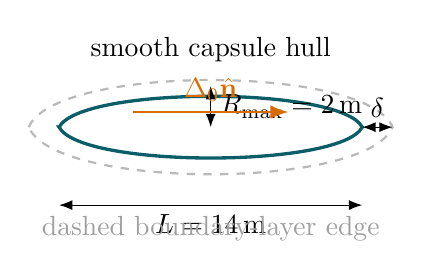
\begin{tikzpicture}[scale=0.55,>=Latex]
	\draw[gray!55,dashed,thick] (-4.2,0) .. controls (-3.6,1.45) and (3.6,1.45) .. (4.2,0) .. controls (3.6,-1.45) and (-3.6,-1.45) .. cycle;
	\draw[accent,very thick] (-3.5,0) .. controls (-3.0,0.95) and (3.0,0.95) .. (3.5,0) .. controls (3.0,-0.95) and (-3.0,-0.95) .. cycle;
	\draw[<->] (-3.5,-1.8) -- (3.5,-1.8) node[midway,below] {$L=14\,\mathrm{m}$};
	\draw[<->] (0,0) -- (0,0.95) node[midway,right] {$R_{\max}=2\,\mathrm{m}$};
	\draw[<->] (3.5,0) -- (4.2,0) node[midway,above] {$\delta$};
	\draw[->,thick,orange!85!black] (-1.8,0.35) -- (1.8,0.35) node[midway,above] {$\Delta_0\hat{\mathbf n}$};
	\node[align=center] at (0,1.8) {smooth capsule hull};
	\node[align=center,gray!75] at (0,-2.35) {dashed boundary-layer edge};
\end{tikzpicture}
\caption{Conceptual capsule geometry used by the model. The solid outline is the hull and the dashed outline marks the displaced-field boundary layer. Dimensions are model parameters, not measurements of a confirmed vehicle.}
\label{fig:capsule_geometry}
\end{figure}

\subsection{Axially Symmetric Capsule Profile}

The craft is modeled as an axially symmetric capsule with longitudinal coordinate $z \in [-L/2, L/2]$ and radial coordinate $r \in [0, R(z)]$. The radius profile $R(z)$ is defined as
\begin{equation}
R(z) = R_{\max} \left[ 1 - \left( \frac{2z}{L} \right)^2 \right]^m,
\end{equation}
where $m \geq 2$ ensures smooth curvature at the endcaps. This profile yields a maximum radius at $z = 0$ and smoothly tapered endcaps at $z = \pm L/2$. The curvature of the hull is given by
\begin{equation}
\kappa_h(z) = \frac{\left| R''(z) \right|}{\left[ 1 + \left( R'(z) \right)^2 \right]^{3/2}},
\end{equation}
which remains finite for all $z$ due to the smoothness of $R(z)$.

\subsection{Hull Smoothness and Curvature Constraints}

To prevent geometric singularities and ensure compatibility with the displacement operator, the hull curvature must satisfy
\begin{equation}
\kappa_h(z) \leq \kappa_{\mathrm{h,max}},
\end{equation}
where $\kappa_{\mathrm{h,max}}$ is an engineering parameter determined by material constraints and boundary-layer stability. The curvature constraint ensures that the hull geometry remains smooth and that the displacement field can be defined without introducing discontinuities or excessive gradients.

The torsion of the hull is identically zero due to axial symmetry:
\begin{equation}
\tau_h(z) = 0,
\end{equation}
which simplifies the construction of the displacement field and stability surfaces.

\subsection{Boundary-Layer Confinement}

A boundary layer of thickness $\delta$ surrounds the hull and defines the region in which the displacement field is nonzero. The boundary-layer radius is given by
\begin{equation}
R_{\mathrm{BL}}(z) = R(z) + \delta.
\end{equation}
Within this region, the displacement field $\Delta(\mathbf{x})$ is confined by a taper function $f(r,z)$ defined as
\begin{equation}
f(r,z) = 1 - \left( \frac{r - R(z)}{\delta} \right)^n,
\qquad
n \geq 2,
\end{equation}
which ensures smooth decay of the displacement amplitude from the hull surface to the boundary-layer edge. The taper function satisfies
\begin{equation}
f(R(z),z) = 1,
\qquad
f(R_{\mathrm{BL}}(z),z) = 0,
\end{equation}
and is differentiable for all $r \in [R(z), R_{\mathrm{BL}}(z)]$.

\subsection{Geometric Cross-Sections}

Cross-sections of the craft at fixed $z$ are circular disks of radius $R(z)$, and cross-sections of the boundary layer are circular disks of radius $R_{\mathrm{BL}}(z)$. The volume of the craft is given by
\begin{equation}
V = \pi \int_{-L/2}^{L/2} R(z)^2 \, dz,
\end{equation}
and the volume of the boundary layer is
\begin{equation}
V_{\mathrm{BL}} = \pi \int_{-L/2}^{L/2} \left[ R_{\mathrm{BL}}(z)^2 - R(z)^2 \right] dz.
\end{equation}
These expressions are used in Section V to normalize the displacement field and in Section VI to construct stability surfaces.

\subsection{Compatibility with Displacement Fields}

The smooth curvature, axial symmetry, and confined boundary layer of the capsule geometry ensure compatibility with the displacement operator defined in Section III. In particular, the smoothness of $R(z)$ and $f(r,z)$ guarantees that the displacement field can be constructed without violating gradient constraints or inducing worldline intersection. The geometric structure established in this section provides the foundation for the displacement-field derivation presented in Section V.
\section{Displacement Field Construction}

The displacement operator introduced in Section III requires a smooth displacement field $\Delta(\mathbf{x})$ confined within the boundary layer defined in Section IV. In this section, we construct the displacement field, establish its amplitude and gradient constraints, and derive the conditions necessary to preserve identity-space coherence under worldline transformation.

\subsection{Displacement Field Definition}

The displacement field is defined as a smooth vector field
\begin{equation}
\Delta : \mathbb{R}^3 \rightarrow \mathbb{R}^3,
\qquad
\Delta(\mathbf{x}) = \Delta_0 \, g(\mathbf{x}) \, f(r,z) \, \hat{\mathbf{n}},
\end{equation}
where $\Delta_0$ is the displacement amplitude, $g(\mathbf{x})$ is a geometric modulation function, $f(r,z)$ is the taper function defined in Section IV, and $\hat{\mathbf{n}}$ is a unit vector specifying the displacement direction. The displacement field is confined to the boundary layer:
\begin{equation}
\Delta(\mathbf{x}) = 0
\qquad
\text{for } r > R_{\mathrm{BL}}(z).
\end{equation}

\subsection{Amplitude and Modulation}

The displacement amplitude $\Delta_0$ is defined as
\begin{equation}
\Delta_0 = \max_{\mathbf{x}} \left\| \Delta(\mathbf{x}) \right\|,
\end{equation}
and represents the maximum displacement applied to worldlines within the boundary layer. The geometric modulation function $g(\mathbf{x})$ is chosen to satisfy
\begin{align}
0 &\leq g(\mathbf{x}) \leq 1, \\
g(\mathbf{x}) &= 1 \text{ on the hull surface}, \\
g(\mathbf{x}) &= 0 \text{ at } r = R_{\mathrm{BL}}(z).
\end{align}
A suitable choice is
\begin{equation}
g(\mathbf{x}) = \exp\left[ -\alpha \left( r - R(z) \right)^2 \right],
\qquad
\alpha > 0,
\end{equation}
which ensures smooth decay of the displacement amplitude away from the hull.

\subsection{Gradient Constraints}

To prevent worldline intersection, the displacement gradient must satisfy
\begin{equation}
\left\| \nabla \Delta(\mathbf{x}) \right\| \leq G_{\max},
\end{equation}
where $G_{\max}$ is a stability-surface parameter determined in Section VI. The gradient of the displacement field is given by
\begin{equation}
\nabla \Delta = 
\Delta_0 \left[
(\nabla g) f \hat{\mathbf{n}}
+
g (\nabla f) \hat{\mathbf{n}}
+
g f (\nabla \hat{\mathbf{n}})
\right].
\end{equation}
Each term must be bounded to ensure smoothness:
\begin{equation}
\left\| \nabla g \right\| \leq C_g,
\qquad
\left\| \nabla f \right\| \leq C_f,
\qquad
\left\| \nabla \hat{\mathbf{n}} \right\| \leq C_n,
\end{equation}
where $C_g$, $C_f$, and $C_n$ are geometric constants determined by the hull curvature and taper function. The gradient constraint becomes
\begin{equation}
\Delta_0 \left( C_g + C_f + C_n \right) \leq G_{\max}.
\end{equation}

\subsection{Worldline Transformation}

Under the displacement operator, worldlines transform according to
\begin{equation}
\gamma'(\tau) = \gamma(\tau) + \Delta\big(\gamma(\tau)\big).
\end{equation}
The tangent vector transforms as
\begin{equation}
\dot{\gamma}'(\tau) = \dot{\gamma}(\tau) + \nabla \Delta\big(\gamma(\tau)\big) \cdot \dot{\gamma}(\tau),
\end{equation}
and the curvature transforms as
\begin{equation}
\kappa' = 
\left\|
\nabla_{\dot{\gamma}'} \dot{\gamma}'
\right\|.
\end{equation}
To preserve identity-space coherence, the transformed curvature must satisfy
\begin{equation}
\kappa' \leq \kappa_{\max},
\end{equation}
where $\kappa_{\max}$ is an engineering parameter determined by the stability surface.

\subsection{Compatibility Conditions}

Compatibility between the displacement field and identity-space requires:
\begin{enumerate}
\item $\Delta(\mathbf{x})$ is smooth and confined to the boundary layer.
\item $\left\| \nabla \Delta \right\|$ satisfies the gradient constraint.
\item $\kappa'$ and $\tau'$ satisfy curvature and torsion limits.
\item Distinct worldlines remain distinct under displacement.
\end{enumerate}
These conditions ensure that the displacement operator does not induce geometric singularities or worldline intersection.

\subsection{Effective Displacement}

The effective displacement per unit ambient time is defined as
\begin{equation}
v_{\mathrm{eff}} = \frac{\Delta_0}{\Delta \tau},
\end{equation}
where $\Delta \tau$ is the ambient time interval over which the displacement is applied. The flight-envelope inequality derived in Section VII imposes bounds on $v_{\mathrm{eff}}$ based on stability-surface parameters and gradient constraints.

The displacement-field construction established in this section provides the foundation for the stability-surface analysis presented in Section VI.
\section{Stability Surfaces and Gradient Limits}

The displacement field constructed in Section V must satisfy stability conditions ensuring that worldlines remain distinct, smooth, and non-intersecting under the action of the displacement operator. These conditions are encoded in the stability surface, which bounds the displacement amplitude, gradient, curvature, and torsion. In this section, we derive the stability-surface equations and establish the gradient limits required for identity-space coherence.

\subsection{Stability Surface Definition}

The stability surface is defined as a hypersurface in identity-space bounding the allowable displacement amplitude and gradient. Let $\mathcal{S}$ denote the stability surface, defined implicitly by
\begin{equation}
F\left( \Delta_0, \left\| \nabla \Delta \right\|, \kappa', \tau' \right) = 0,
\end{equation}
where $F$ is a smooth function satisfying
\begin{equation}
F < 0 \quad \text{stable}, \qquad F = 0 \quad \text{critical}, \qquad F > 0 \quad \text{unstable}.
\end{equation}
The stability surface imposes the constraints
\begin{equation}
\Delta_0 \leq \Delta_S,
\qquad
\left\| \nabla \Delta \right\| \leq G_{\max},
\qquad
\kappa' \leq \kappa_{\max},
\qquad
\tau' \leq \tau_{\max},
\end{equation}
where $\Delta_S$, $G_{\max}$, $\kappa_{\max}$, and $\tau_{\max}$ are engineering parameters determined by the boundary-layer structure and displacement-field geometry.

\subsection{Displacement-Amplitude Bound}

The displacement amplitude must satisfy
\begin{equation}
\Delta_0 \leq \Delta_S,
\end{equation}
where $\Delta_S$ is the stability amplitude. The stability amplitude is defined as
\begin{equation}
\Delta_S = \min_{\mathbf{x}} \left[ \frac{1}{C_g + C_f + C_n} G_{\max} \right],
\end{equation}
ensuring that the gradient constraint is satisfied for all points within the boundary layer. This bound prevents excessive displacement that could induce worldline intersection or curvature singularities.

\subsection{Gradient Limit}

The gradient limit is derived from the requirement that worldlines remain distinct under displacement. The displacement gradient must satisfy
\begin{equation}
\left\| \nabla \Delta(\mathbf{x}) \right\| \leq G_{\max},
\end{equation}
where $G_{\max}$ is determined by the stability surface. Substituting the expression for $\nabla \Delta$ from Section V yields
\begin{equation}
\Delta_0 \left( C_g + C_f + C_n \right) \leq G_{\max}.
\end{equation}
This inequality ensures that the displacement field does not collapse distinct worldlines into a single identity-space location.

\subsection{Worldline Non-Intersection Inequality}

Identity-space coherence requires that distinct worldlines remain distinct under displacement. Let $\gamma_1$ and $\gamma_2$ be two worldlines with initial separation
\begin{equation}
d_0 = \left\| \gamma_1(\tau) - \gamma_2(\tau) \right\|.
\end{equation}
Under displacement, the separation becomes
\begin{equation}
d' = \left\| \gamma_1'(\tau) - \gamma_2'(\tau) \right\|
= \left\| d_0 + \Delta(\gamma_1) - \Delta(\gamma_2) \right\|.
\end{equation}
To prevent intersection, we require
\begin{equation}
d' \geq \epsilon d_0,
\qquad
\epsilon > 0.
\end{equation}
This condition is satisfied if
\begin{equation}
\left\| \Delta(\gamma_1) - \Delta(\gamma_2) \right\|
\geq
(\epsilon - 1) d_0,
\end{equation}
which imposes a lower bound on the displacement gradient:
\begin{equation}
\left\| \nabla \Delta \right\| \geq \epsilon - 1.
\end{equation}
Combined with the upper bound, the gradient must satisfy
\begin{equation}
\epsilon - 1 \leq \left\| \nabla \Delta \right\| \leq G_{\max}.
\end{equation}

\subsection{Curvature Stability}

The curvature of displaced worldlines must satisfy
\begin{equation}
\kappa' = 
\left\|
\nabla_{\dot{\gamma}'} \dot{\gamma}'
\right\|
\leq \kappa_{\max},
\end{equation}
where $\kappa_{\max}$ is determined by the boundary-layer geometry and displacement amplitude. Substituting the expression for $\dot{\gamma}'$ yields
\begin{equation}
\kappa' \leq 
\left\|
\nabla_{\dot{\gamma}} \dot{\gamma}
\right\|
+
\left\|
\nabla_{\dot{\gamma}} \left( \nabla \Delta \cdot \dot{\gamma} \right)
\right\|.
\end{equation}
The curvature stability condition becomes
\begin{equation}
\kappa + \Delta_0 (C_g + C_f + C_n) \leq \kappa_{\max}.
\end{equation}

\subsection{Torsion Stability}

The torsion of displaced worldlines must satisfy
\begin{equation}
\tau' \leq \tau_{\max},
\end{equation}
where $\tau_{\max}$ is an engineering parameter determined by the boundary-layer structure. The torsion transforms according to
\begin{equation}
\tau' = \tau + \left\langle \nabla_{\dot{\gamma}} B, \nabla \Delta \cdot N \right\rangle,
\end{equation}
yielding the stability condition
\begin{equation}
\tau + \Delta_0 C_n \leq \tau_{\max}.
\end{equation}

\subsection{Stability-Surface Summary}

The stability surface imposes the combined constraints
\begin{equation}
\Delta_0 \leq \Delta_S,
\qquad
\left\| \nabla \Delta \right\| \leq G_{\max},
\qquad
\kappa' \leq \kappa_{\max},
\qquad
\tau' \leq \tau_{\max},
\end{equation}
ensuring that the displacement operator preserves identity-space coherence and prevents geometric singularities. These constraints form the basis for the flight-envelope inequality derived in Section VII. Their joint admissible region is illustrated schematically in Fig.~\ref{fig:stability_surface}.
\begin{figure}[tb]
\centering
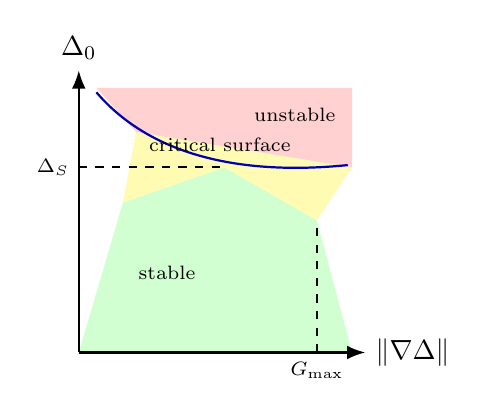
\begin{tikzpicture}[scale=0.56,>=Latex]
	\fill[green!18] (0,0) -- (6.2,0) -- (5.4,3.0) -- (3.3,4.2) -- (1.0,3.4) -- cycle;
	\fill[yellow!30] (1.0,3.4) -- (3.3,4.2) -- (5.4,3.0) -- (6.2,4.2) -- (1.3,5.0) -- cycle;
	\fill[red!18] (1.3,5.0) -- (6.2,4.2) -- (6.2,6.0) -- (0.4,6.0) -- cycle;
	\draw[thick,->] (0,0) -- (6.5,0) node[right] {$\|\nabla\Delta\|$};
	\draw[thick,->] (0,0) -- (0,6.4) node[above] {$\Delta_0$};
	\draw[thick,blue!70!black] (0.4,5.9) .. controls (1.6,4.5) and (3.6,4.0) .. (6.1,4.25);
	\draw[dashed,thick] (5.4,0) -- (5.4,3.0);
	\draw[dashed,thick] (0,4.2) -- (3.3,4.2);
	\node[font=\scriptsize] at (2.0,1.8) {stable};
	\node[font=\scriptsize] at (3.2,4.7) {critical surface};
	\node[font=\scriptsize] at (4.9,5.4) {unstable};
	\node[font=\scriptsize,below] at (5.4,0) {$G_{\max}$};
	\node[font=\scriptsize,left] at (0,4.2) {$\Delta_S$};
\end{tikzpicture}
\caption{Schematic stability surface in displacement-amplitude/gradient space. The colored regions communicate the model logic: admissible operation lies below both the amplitude and gradient bounds, while the boundary is a critical operating surface.}
\label{fig:stability_surface}
\end{figure}
\section{Flight-Envelope Inequality}

The displacement field and stability-surface constraints derived in Sections V and VI impose bounds on the effective displacement per unit ambient time. These bounds define the flight envelope of the displacement-based vehicle. In this section, we derive the flight-envelope inequality, which specifies the allowable range of effective displacement velocities consistent with identity-space coherence, gradient limits, and curvature stability.

\subsection{Effective Displacement Velocity}

The effective displacement velocity is defined as
\begin{equation}
v_{\mathrm{eff}} = \frac{\Delta_0}{\Delta \tau},
\end{equation}
where $\Delta_0$ is the displacement amplitude and $\Delta \tau$ is the ambient time interval over which the displacement is applied. This quantity represents the apparent motion of the vehicle as observed in ambient space, although the underlying mechanism is a geometric displacement of worldlines in identity-space.

\subsection{Upper Bound from Stability Surface}

The stability surface imposes the constraint
\begin{equation}
\Delta_0 \leq \Delta_S,
\end{equation}
where $\Delta_S$ is the stability amplitude. Substituting this into the definition of $v_{\mathrm{eff}}$ yields the upper bound
\begin{equation}
v_{\mathrm{eff}} \leq \frac{\Delta_S}{\Delta \tau}.
\end{equation}
This bound ensures that the displacement amplitude does not exceed the stability limit imposed by gradient, curvature, and torsion constraints.

\subsection{Upper Bound from Gradient Limit}

The gradient limit derived in Section VI imposes the constraint
\begin{equation}
\Delta_0 \left( C_g + C_f + C_n \right) \leq G_{\max}.
\end{equation}
Solving for $\Delta_0$ yields
\begin{equation}
\Delta_0 \leq \frac{G_{\max}}{C_g + C_f + C_n}.
\end{equation}
Substituting into the definition of $v_{\mathrm{eff}}$ yields the gradient-limited upper bound
\begin{equation}
v_{\mathrm{eff}} \leq \frac{G_{\max}}{(C_g + C_f + C_n)\Delta \tau}.
\end{equation}

\subsection{Lower Bound from Non-Intersection Constraint}

The worldline non-intersection inequality derived in Section VI imposes the constraint
\begin{equation}
\left\| \nabla \Delta \right\| \geq \epsilon - 1,
\end{equation}
which yields the lower bound
\begin{equation}
\Delta_0 \geq \frac{\epsilon - 1}{C_g + C_f + C_n}.
\end{equation}
Substituting into the definition of $v_{\mathrm{eff}}$ yields
\begin{equation}
v_{\mathrm{eff}} \geq \frac{\epsilon - 1}{(C_g + C_f + C_n)\Delta \tau}.
\end{equation}
This bound ensures that the displacement field maintains sufficient gradient to preserve worldline separation.

\subsection{Combined Flight-Envelope Inequality}

Combining the upper and lower bounds yields the flight-envelope inequality
\begin{equation}
\frac{\epsilon - 1}{(C_g + C_f + C_n)\Delta \tau}
\leq
v_{\mathrm{eff}}
\leq
\min\left[
\frac{\Delta_S}{\Delta \tau},
\frac{G_{\max}}{(C_g + C_f + C_n)\Delta \tau}
\right].
\end{equation}
This inequality specifies the allowable range of effective displacement velocities consistent with identity-space coherence, gradient limits, and curvature stability.

\subsection{Engineering Interpretation}

The flight-envelope inequality provides a quantitative specification for the operational limits of the displacement-based vehicle. The lower bound ensures that the displacement field maintains sufficient gradient to preserve worldline separation, while the upper bound ensures that the displacement amplitude and gradient remain within stability-surface limits. The inequality thus defines the allowable range of effective motion and provides a basis for engineering analysis and system design.

The flight-envelope inequality derived in this section forms the foundation for the engineering requirements and operational considerations presented in Section VIII. Figure~\ref{fig:highlight_image} summarizes the proposed geometry-to-envelope workflow.
\section{Engineering Requirements and Operational Considerations}

The displacement-field model and flight-envelope inequality derived in the preceding sections impose explicit engineering requirements on the design and operation of a displacement-based vehicle. These requirements ensure that the displacement operator preserves identity-space coherence, maintains boundary-layer stability, and satisfies curvature and torsion limits. In this section, we summarize the engineering constraints and discuss their implications for system design and operational behavior.

\subsection{Displacement-Amplitude Requirements}

The displacement amplitude $\Delta_0$ must satisfy the stability-surface constraint
\begin{equation}
\Delta_0 \leq \Delta_S,
\end{equation}
where $\Delta_S$ is determined by the gradient limit and boundary-layer geometry. The amplitude must also satisfy the gradient-limited bound
\begin{equation}
\Delta_0 \leq \frac{G_{\max}}{C_g + C_f + C_n}.
\end{equation}
These constraints ensure that the displacement field remains smooth and does not induce excessive curvature or torsion in displaced worldlines. The displacement amplitude must be selected to satisfy both bounds simultaneously.

\subsection{Boundary-Layer Tolerances}

The boundary layer of thickness $\delta$ surrounding the hull defines the region in which the displacement field is nonzero. The taper function $f(r,z)$ must satisfy
\begin{equation}
f(R(z),z) = 1,
\qquad
f(R_{\mathrm{BL}}(z),z) = 0,
\end{equation}
and must be differentiable for all $r \in [R(z), R_{\mathrm{BL}}(z)]$. The geometric modulation function $g(\mathbf{x})$ must satisfy
\begin{equation}
0 \leq g(\mathbf{x}) \leq 1,
\end{equation}
and must decay smoothly away from the hull surface. These conditions ensure that the displacement field is confined to the boundary layer and that the gradient remains within allowable limits.

\subsection{Curvature and Torsion Limits}

The curvature and torsion of displaced worldlines must satisfy
\begin{equation}
\kappa' \leq \kappa_{\max},
\qquad
\tau' \leq \tau_{\max},
\end{equation}
where $\kappa_{\max}$ and $\tau_{\max}$ are engineering parameters determined by the boundary-layer geometry and displacement amplitude. These limits ensure that the displacement operator does not induce excessive bending or twisting of worldlines, preserving geometric smoothness and identity-space coherence.

\subsection{Gradient Stability}

The displacement gradient must satisfy the combined bounds
\begin{equation}
\epsilon - 1 \leq \left\| \nabla \Delta \right\| \leq G_{\max},
\end{equation}
ensuring that the displacement field maintains sufficient gradient to preserve worldline separation while remaining within stability-surface limits. The gradient stability condition imposes constraints on the taper function, geometric modulation function, and displacement amplitude.

\subsection{Operational Envelope}

The flight-envelope inequality derived in Section VII imposes the operational constraint
\begin{equation}
\frac{\epsilon - 1}{(C_g + C_f + C_n)\Delta \tau}
\leq
v_{\mathrm{eff}}
\leq
\min\left[
\frac{\Delta_S}{\Delta \tau},
\frac{G_{\max}}{(C_g + C_f + C_n)\Delta \tau}
\right].
\end{equation}
This inequality specifies the allowable range of effective displacement velocities consistent with identity-space coherence, gradient limits, and curvature stability. The operational envelope must be respected to ensure stable and coherent displacement-based motion.

\subsection{System-Level Considerations}

The engineering requirements derived in this section impose constraints on system design, including:
\begin{enumerate}
\item The displacement amplitude must be selected to satisfy stability-surface and gradient limits.
\item The boundary-layer geometry must be designed to ensure smooth tapering and gradient stability.
\item The curvature and torsion limits must be respected to prevent geometric singularities.
\item The operational envelope must be enforced to ensure stable displacement-based motion.
\end{enumerate}
These considerations provide a basis for engineering analysis and system design, ensuring that the displacement-based vehicle operates within allowable limits and maintains identity-space coherence.

The engineering requirements and operational considerations presented in this section form the foundation for the geometric specifications and parameter tables provided in the Appendix.
\section{Conclusion}

This work has presented a displacement-based warp-field model constructed within the identity-space formalism of SEFI, DEFI, and GWFM. Motivated by publicly reported aerospace observations describing smooth, capsule-like craft exhibiting extreme kinematic profiles, the model treats the tic-tac geometry as a well-defined engineering object with smooth curvature, confined boundary-layer structure, and displacement-field compatibility. The geometric framework developed in Section III provides the foundation for constructing smooth displacement operators acting on worldlines in identity-space, enabling effective motion without reliance on exotic stress-energy tensors or metric engineering.

The displacement field derived in Section V satisfies gradient, curvature, and torsion constraints imposed by the stability surface defined in Section VI. These constraints ensure that worldlines remain distinct, smooth, and non-intersecting under displacement. The flight-envelope inequality derived in Section VII imposes bounds on effective displacement velocity, providing a quantitative specification for allowable operational behavior. The engineering requirements summarized in Section VIII translate these mathematical constraints into explicit system-level considerations, including displacement amplitude limits, boundary-layer tolerances, curvature and torsion stability, and operational envelope enforcement.

The resulting framework provides a mathematically coherent engineering specification for a displacement-based vehicle, suitable for evaluation, critique, and extension by researchers in geometric field theory, aerospace engineering, and applied physics. The model demonstrates that displacement-based motion can be represented within a smooth geometric structure without violating identity-space coherence or inducing geometric singularities. Future work may explore extensions of the displacement operator, alternative boundary-layer geometries, and applications of the stability-surface formalism to multi-entity systems.

The geometric specifications and parameter tables provided in the Appendix support engineering analysis and system design, ensuring that the displacement-based vehicle operates within allowable limits and maintains identity-space coherence.
\begin{figure*}[tb]
\centering
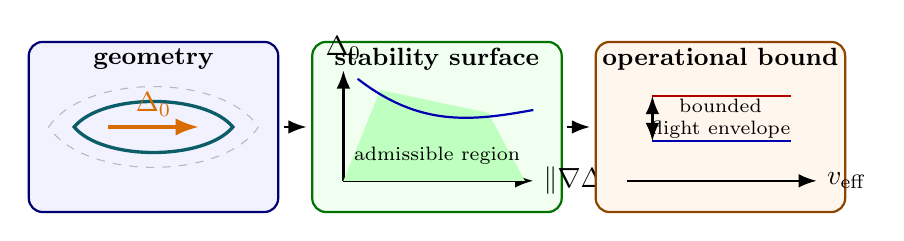
\begin{tikzpicture}[scale=0.72,>=Latex]
	\draw[rounded corners=5pt,fill=blue!5,draw=blue!45!black,thick] (0,0) rectangle (4.4,3.0);
	\draw[gray!55,dashed] (0.35,1.5) .. controls (1.0,2.45) and (3.4,2.45) .. (4.05,1.5) .. controls (3.4,0.55) and (1.0,0.55) .. cycle;
	\draw[accent,very thick] (0.8,1.5) .. controls (1.3,2.1) and (3.1,2.1) .. (3.6,1.5) .. controls (3.1,0.9) and (1.3,0.9) .. cycle;
	\draw[->,orange!85!black,very thick] (1.4,1.5) -- (3.0,1.5) node[midway,above] {$\Delta_0$};
	\node[font=\small\bfseries] at (2.2,2.7) {geometry};
	\draw[rounded corners=5pt,fill=green!6,draw=green!45!black,thick] (5.0,0) rectangle (9.4,3.0);
	\draw[->,thick] (5.55,0.55) -- (8.9,0.55) node[right] {$\|\nabla\Delta\|$};
	\draw[->,thick] (5.55,0.55) -- (5.55,2.5) node[above] {$\Delta_0$};
	\fill[green!25] (5.55,0.55) -- (8.75,0.55) -- (8.1,1.75) -- (6.2,2.15) -- cycle;
	\draw[blue!70!black,thick] (5.8,2.35) .. controls (6.9,1.5) and (7.8,1.6) .. (8.9,1.8);
	\node[font=\small\bfseries] at (7.2,2.7) {stability surface};
	\node[font=\scriptsize] at (7.2,1.0) {admissible region};
	\draw[rounded corners=5pt,fill=orange!7,draw=orange!55!black,thick] (10.0,0) rectangle (14.4,3.0);
	\draw[->,thick] (10.55,0.55) -- (13.9,0.55) node[right] {$v_{\mathrm{eff}}$};
	\draw[thick,blue!70!black] (11.0,1.25) -- (13.45,1.25);
	\draw[thick,red!70!black] (11.0,2.05) -- (13.45,2.05);
	\draw[<->,thick] (11.0,1.25) -- (11.0,2.05);
	\node[font=\scriptsize,align=center] at (12.2,1.65) {bounded\\flight envelope};
	\node[font=\small\bfseries] at (12.2,2.7) {operational bound};
	\draw[->,thick] (4.5,1.5) -- (4.9,1.5);
	\draw[->,thick] (9.5,1.5) -- (9.9,1.5);
\end{tikzpicture}
\caption{Highlight image for the proposed framework. The model proceeds from a smooth capsule and confined displacement field, through a bounded stability surface, to an operational flight-envelope inequality. This image is a conceptual synthesis of the equations in the paper, not an experimental photograph or performance claim.}
\label{fig:highlight_image}
\end{figure*}
\appendix
\section{Engineering Specifications and Parameter Tables}
\subsection{Geometric Parameters}

\begin{table}[h!]
\centering
\begin{tabular}{l c}
\hline
Parameter & Value \\
\hline
Craft length $L$ & $14\,\mathrm{m}$ \\
Maximum radius $R_{\max}$ & $2\,\mathrm{m}$ \\
Boundary-layer thickness $\delta$ & $1\,\mathrm{m}$ \\
Endcap smoothness exponent $m$ & $\geq 2$ \\
Boundary-layer taper exponent $n$ & $\geq 2$ \\
Hull curvature limit $\kappa_{\mathrm{h,max}}$ & Engineering parameter \\
\hline
\end{tabular}
\caption{Geometric parameters defining the tic-tac capsule profile.}
\end{table}

\subsection{Boundary-Layer Parameters}

\begin{table}[h!]
\centering
\begin{tabular}{l c}
\hline
Parameter & Definition \\
\hline
Boundary-layer radius $R_{\mathrm{BL}}(z)$ & $R(z) + \delta$ \\
Taper function $f(r,z)$ & $1 - \left( \frac{r - R(z)}{\delta} \right)^n$ \\
Modulation function $g(\mathbf{x})$ & $\exp\left[ -\alpha (r - R(z))^2 \right]$ \\
Modulation constant $\alpha$ & $> 0$ \\
\hline
\end{tabular}
\caption{Boundary-layer parameters and taper functions.}
\end{table}

\subsection{Displacement-Field Constants}

\begin{table}[h!]
\centering
\begin{tabular}{l c}
\hline
Constant & Description \\
\hline
$\Delta_0$ & Displacement amplitude \\
$C_g$ & Gradient bound from modulation function \\
$C_f$ & Gradient bound from taper function \\
$C_n$ & Gradient bound from displacement direction \\
$G_{\max}$ & Maximum allowable displacement gradient \\
$\Delta_S$ & Stability amplitude \\
\hline
\end{tabular}
\caption{Constants governing displacement-field stability.}
\end{table}

\subsection{Stability-Surface Parameters}

\begin{table}[h!]
\centering
\begin{tabular}{l c}
\hline
Parameter & Constraint \\
\hline
Displacement amplitude & $\Delta_0 \leq \Delta_S$ \\
Gradient limit & $\left\| \nabla \Delta \right\| \leq G_{\max}$ \\
Curvature limit & $\kappa' \leq \kappa_{\max}$ \\
Torsion limit & $\tau' \leq \tau_{\max}$ \\
Non-intersection bound & $d' \geq \epsilon d_0$ \\
\hline
\end{tabular}
\caption{Stability-surface constraints.}
\end{table}

\subsection{Flight-Envelope Constants}

\begin{table}[h!]
\centering
\begin{tabular}{l c}
\hline
Constant & Definition \\
\hline
Effective displacement velocity $v_{\mathrm{eff}}$ & $\Delta_0 / \Delta \tau$ \\
Lower bound & $(\epsilon - 1)/[(C_g + C_f + C_n)\Delta \tau]$ \\
Upper bound (stability) & $\Delta_S / \Delta \tau$ \\
Upper bound (gradient) & $G_{\max}/[(C_g + C_f + C_n)\Delta \tau]$ \\
\hline
\end{tabular}
\caption{Constants defining the flight-envelope inequality.}
\end{table}
\section*{Acknowledgments}

The author acknowledges constructive discussions with colleagues in geometric field theory and aerospace engineering, and the broader scientific community whose interest in unconventional motion signatures has motivated the development of displacement-based geometric models. The SEFI, DEFI, and GWFM frameworks were developed independently, with DEFI introduced in the submitted manuscript \textit{Unified Geometric Field Theory from Worldline and Identity-Space Invariants}~\cite{DuttonUnified2026}, and together form the mathematical foundation of this work.

\begin{thebibliography}{5}
\bibitem{NASA2023UAP}
NASA, \textit{Unidentified Anomalous Phenomena Independent Study Team Report} (2023),
\url{https://science.nasa.gov/uap/}.

\bibitem{DuttonSEFI2026}
J. Dutton, \textit{SEFI: The Single Entity Field Interpretation} (2026), independent research manuscript,\
\url{https://github.com/JasonSEFIDEFI/SEFI-Manuscripts}.

\bibitem{DuttonGWFM2026}
J. Dutton, \textit{Geometric Worldline Foundations of the Electron Field} (2026), independent research manuscript,\
\url{https://github.com/JasonSEFIDEFI/SEFI-Manuscripts}.

\bibitem{DuttonUnified2026}
J. Dutton, \textit{Unified Geometric Field Theory from Worldline and Identity-Space Invariants} (2026), submitted manuscript.

\bibitem{Alcubierre1994}
M. Alcubierre, Classical and Quantum Gravity \textbf{11}, L73 (1994),\
doi:10.1088/0264-9381/11/5/001.

\bibitem{MorrisThorne1988}
M. S. Morris and K. S. Thorne, American Journal of Physics \textbf{56}, 395 (1988),\
doi:10.1119/1.15620.
\end{thebibliography}

\end{document}
